
%Rodzia� 4
\newpage
\chapter{Sterowanie w przestrzeni przegub�w - Kuba}
  \section{Serwomechanizmy przegub�w}
  \section{Sterowanie w przestrzeni przegub�w}
  
  \subsection{Metoda odwrotnego modelu}
  Jedn? z najbardziej popularnych metod sterowania pozycyjnego w robotyce jest metoda odwrotnego modelu. Metoda modelu odwrotnego jest stosowan? w robotyce metod? linearyzacji i dekompozycji modelu matematycznego manipulatora, dzi?ki kt�rej mo?na sterowa? niezale?nie wszystkimi ramionami robota z wykorzystaniem technik sterowania obiektami liniowymi. Metoda odwrotnego modelu ma t? zalet? w por�wnaniu z innymi metodami linearyzacji (np. rozwini?cie w szereg Taylora) modelu, ?e kompensuje nieliniowo?ci w ca?ym zakresie zmian wsp�?rz?dnych z??czowych, a nie tylko w pobli?u punktu, wok�? kt�rego linearyzujemy model. 
    
  Na rys. \ref{rys:4_1} przedstawiony jest og�lny schemat sterowania robota (mechanizmu wielocz?onowego) z wykorzystanim modelu odwrotnego.
  %
    \begin{figure}[htb!]
  	\begin{center}
  		\includegraphics[width=1\linewidth]{figures/fig4_1}
  		\caption{Schemat sterowania robota z wykorzystaniem modelu odwrotnego}\label{rys:4.1}
  	\end{center}
  \end{figure}

W strukturze sterowania mo?emy wyr�?ni? dwie p?tle sprz??enia zwrotnego:
%
\begin{itemize}
\item	P?tl? wewn?trzn? linearyzuj?c? i rozdzielaj?ca prawo sterowania na cze?? modelow? oraz sprz??eniow?
\item	P?tl? zewn?trzn? sprz??enia zwrotnego pozwalaj?c? na sterowanie manipulatora w ??dany spos�b
\end{itemize}
%
Aby wyznaczy? odpowiednie sygna?y steruj?ce, nale?y wszystkie uk?ady zwi?zane z przegubami uniezale?ni? od siebie. Pozwoli to na uproszczenie problemu wyznaczenia sterowania do wyznaczenia sygna?�w steruj?cych dla sze?ciu odsprz?gni?tych uk?ad�w drugiego rz?du. Metody odsprz?gania przegub�w robota opisano m.in. w \cite{fu:1987}, \cite{craig:1995}.

Dany jest model robota opisany r�wnaniem \ref{eq:10}. Przyjmuj?c posta? wektora sygna?�w steruj?cych:
\begin{equation}
	\tau=P(x,t)\hat{\tau}+R(x,t),
\end{equation}\label{eq:4_1}
oraz przyjmuj?c, ?e:
\begin{equation}
P(x,t)=\hat{M}(x,t)
\end{equation}\label{eq:4_2}
%
\begin{equation}
R(x,t)=\hat{V}(x,t)+\hat{G}(x,t)
\end{equation}\label{eq:4_3}
%
mo?na rozdzieli? uk?ady zwi?zane z przegubami w r�wnaniu (\ref{eq:10}). Macierze $\hat{M}(x,t)$, $\hat{V}(x,t)$,$\hat{G}(x,t)$ s? oszacowaniami (estymatami) macierzy $M(x,t)$, $V(x,t)$,$G(x,t)$, w r�wnaniach Lagrange?a-Eulera, liczonymi wed?ug wzor�w podanych w rozdziale 1, na podstawie oszacowanych parametr�w robota. 

R�wnanie opisuj?ce dynamik? robota mo?na zapisa?, wykorzystuj?c
zale?no?ci (3.10) i (\ref{eq:4_1}), w postaci:
%
\begin{equation}
M(x,t)\ddot{q}+G(x)+V(x)=P(x,t)\hat{\tau}+R(x)
\end{equation}\label{eq:4_4}
%
Zak?adaj?c, ?e oszacowane parametry robota maj? te same warto?ci co parametry rzeczywiste,
r�wnanie (\ref{eq:4_4}) upraszcza si? do postaci:
%
\begin{equation}
M(x,t)\ddot{q}=\hat{M}(x,t)\hat{\tau}
\end{equation}\label{eq:4_5}
%
Zak?adaj?c, ?e macierz $M(x)$ jest macierz? nieosobliw?, oraz $M(x)= \hat{M}(x)$, w
wyniku odsprz?gni?cia uzyskuje si? sze?? niezale?nych uk?ad�w opisanych r�wnaniami drugiego rz?du, postaci:
%
\begin{equation}
\ddot{q}=\hat{\tau}
\end{equation}\label{eq:4_6}
%
Uk?ad (\ref{eq:4_6}) mo?na opisa? r�wnaniami w przestrzeni zmiennych stanu jako
%:
\begin{equation}
	\left\{\begin{array}{l}
	\dot{x_{i}}=Ax_{i}+B\hat{tau}\\
	y_{i}=Cx_{i}\\
	i=1,\dots,n
	\end{array}\right.
\end{equation}\label{eq:4_7}
gdzie
\begin{equation}
x_{i}=\left[\begin{array}{c}
q_{i}\\
\dot{q_{i}}
\end{array}\right],
A=\left[\begin{array}{cc}
0 & 1\\
0 & 0
\end{array}\right],
B=\left[\begin{array}{c}
0\\
1
\end{array}\right],
c=\left[1 \quad 0\right],
\end{equation}\label{eq:4_8}
%
G?�wnym wymaganiem przy stosowaniu metody odwrotnego modelu do sterowania jest konieczno?? zapewnienia dok?adnych oraz szybkich pomiar�w wsp�?rz?dnych z??czowych. Jest to silne za?o?enie, poniewa? pomiar parametr�w robota jest zawsze obarczony jest pewnym b??dem to nie wszystkie parametry modelu s? dok?adnie okre?lone. 
    \subsection{Transmitancja przegubu - Kuba}
    \subsection{Regulator po�o�enia przegubu - Kuba}
    \subsection{Regulator momentu przegubu - Janek}
    \subsection{Stabilno�� uk�adu regulacji i wska�niki jako�ci regulacji - Kuba}
  \section{Sterowanie adaptacyjne - Kuba}
%-----
